% \cleardoublepage
\chapter{Plan and Timeline}\minitoc\label{sec:plan}\vspace{.5cm}

\section{Project Plan}

During the development phase, we adhere to the rapid prototyping model \Cref{fig:plan:rapid_prototyping_software}. 
This approach involves starting with a high-level architecture rather than a detailed, concrete design. 
The focus is on breaking down features and components into tasks, allowing for agile and iterative development. 
This approach enables us to quickly prototype and test different functionalities, leading to efficient development and flexibility in the design process.
Each task is designed to be self-contained and independent, allowing for development and testing within the existing code base. 
The development process follows a loop of building prototypes, reviewing them, refining the implementation, and iterating on the design. 
The goal is to complete each task within a time frame of 1-2 weeks, ensuring a focused and efficient development process. This iterative approach allows for rapid progress and continuous improvement throughout the project.

\begin{figure}[H]
	\centering
	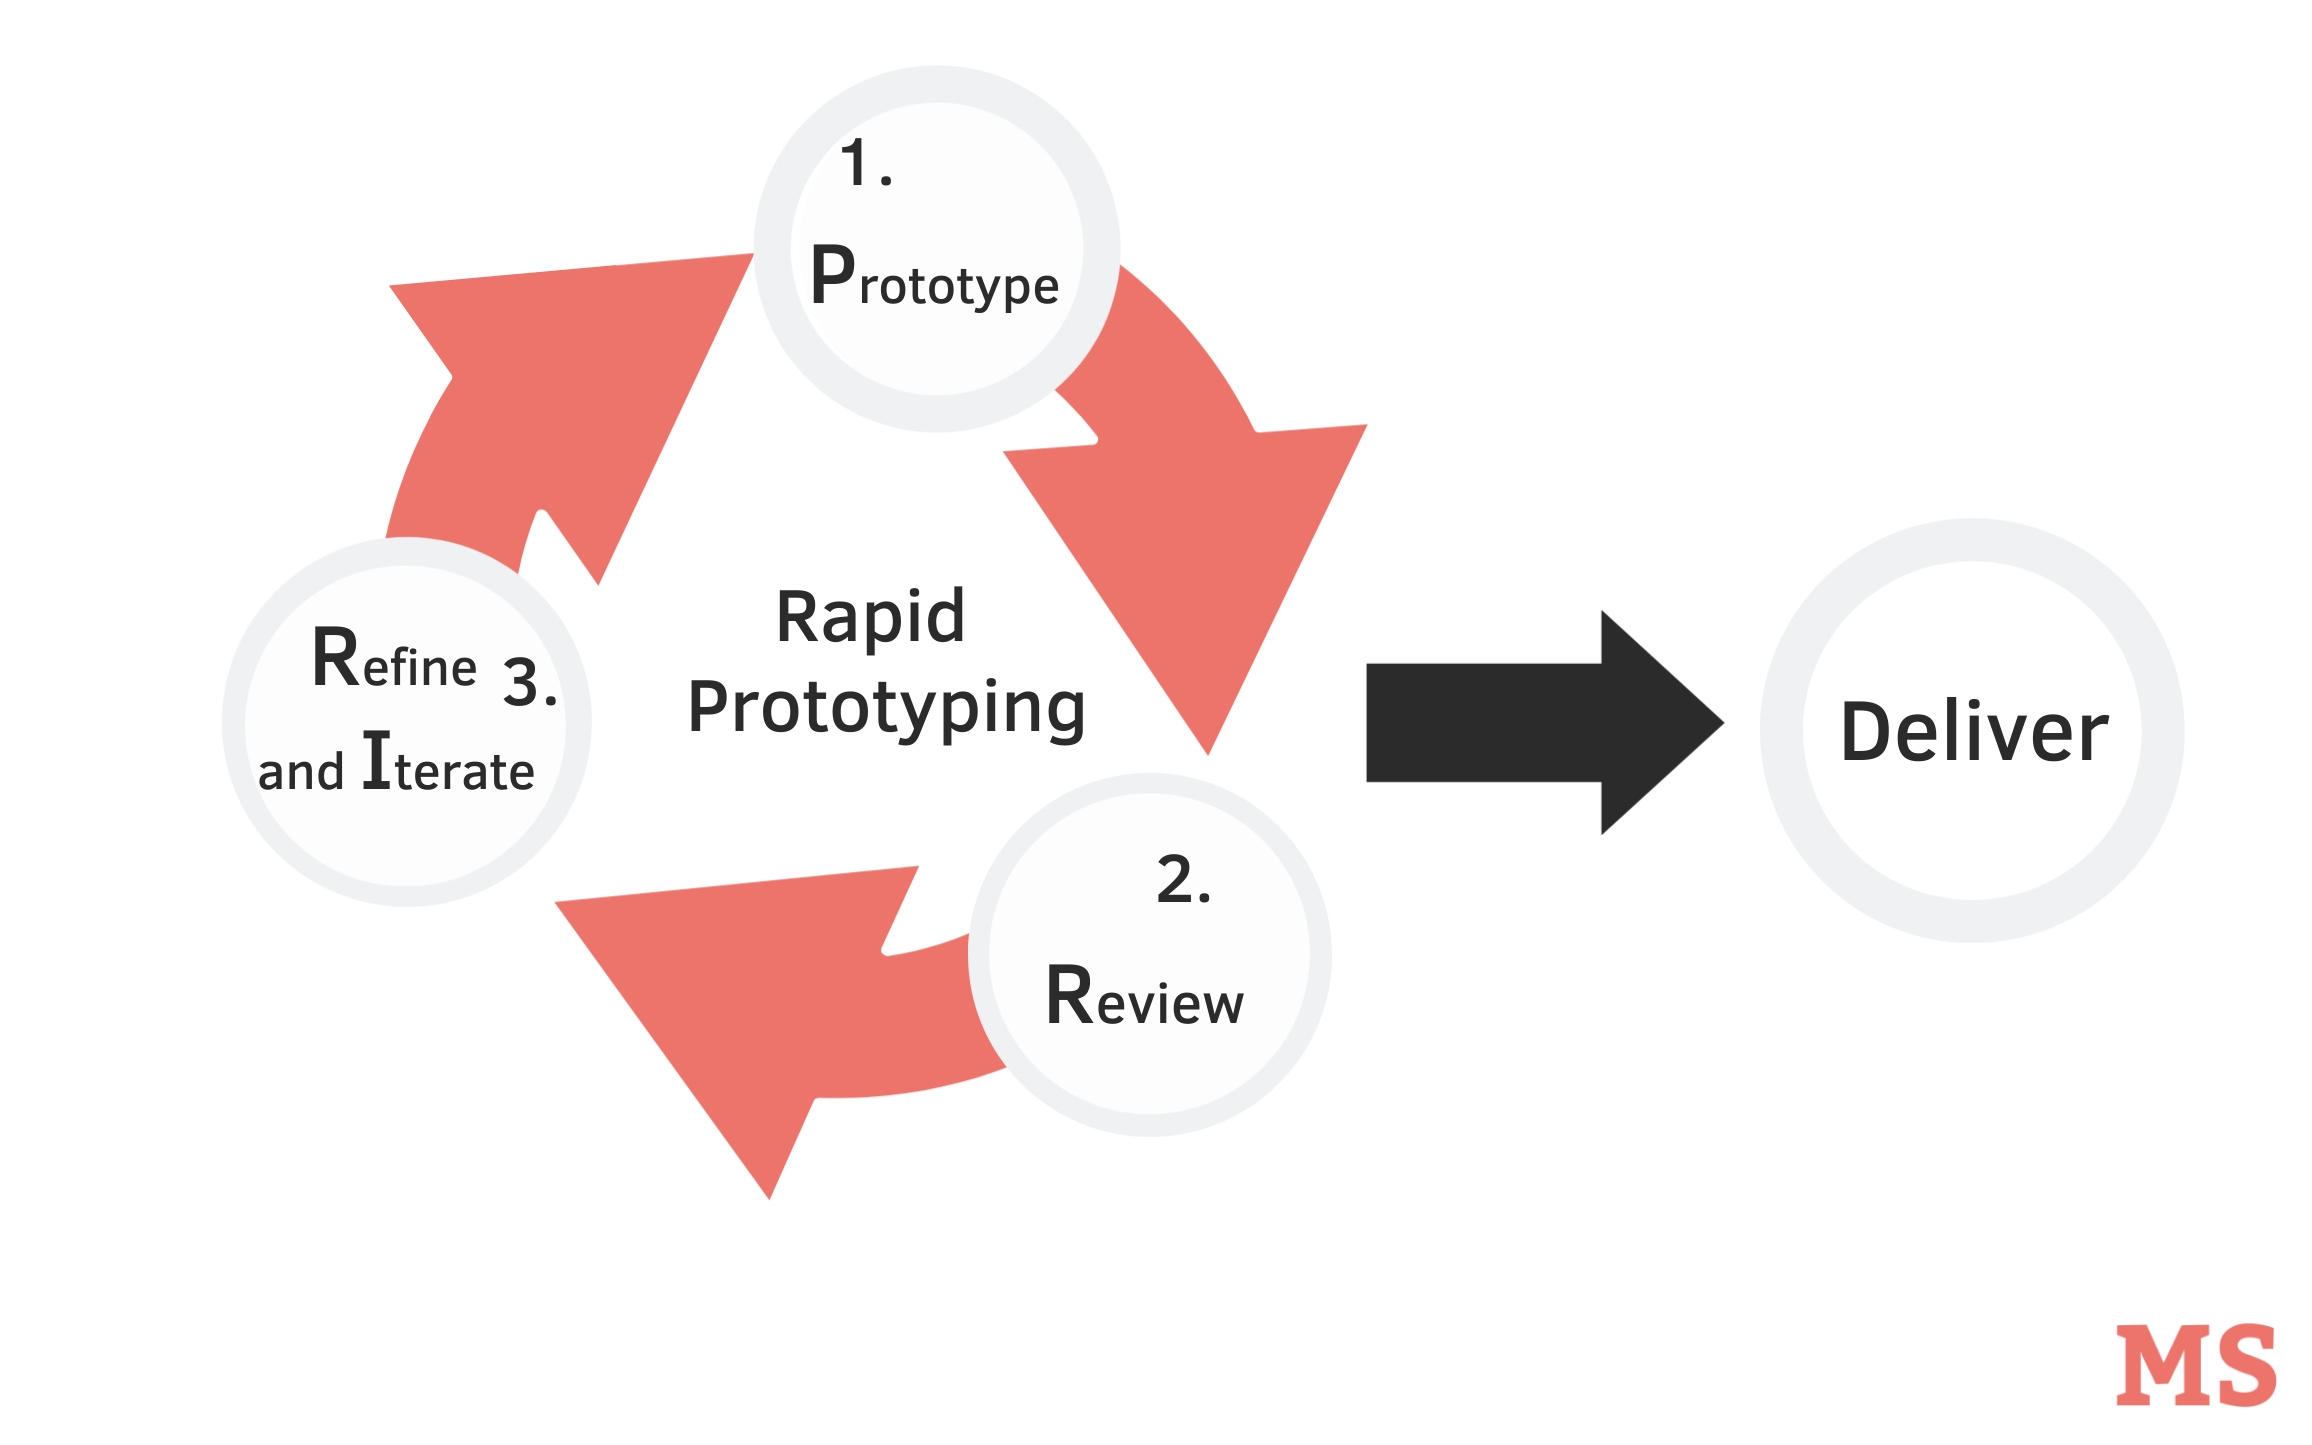
\includegraphics[width=1.0\textwidth]{rapid_prototyping_software.png}
	\caption{Rapid prototyping cycle \cite{marketsplash_rapid_2021}}
	\label{fig:plan:rapid_prototyping_software}
\end{figure}

The development process will take place within a Linux environment. 
As for testing purposes, the program binary will be deployed and executed on 2 industrial-grade computers \textit{UP CORE} designed by \ac{AAEON}, equipped with multiple Ethernet ports \cite{upc_core} \cite{upc_extension_board}. 
The binary will establish a tunnel between two UPC machines using three specific Ethernet ports. 
It's important to note that the fourth port is unrelated to the multipath tunneling and is solely used for remote management purposes.
The UPC machines, equipped with this library, can be utilized as part of the AV's 5G test bed. 
In this setup, RAN (Radio Access Network) and Open5GS software will be installed on the UPC machines, enabling comprehensive testing and evaluation of 5G functionalities.

\begin{figure}[H]
	\centering
	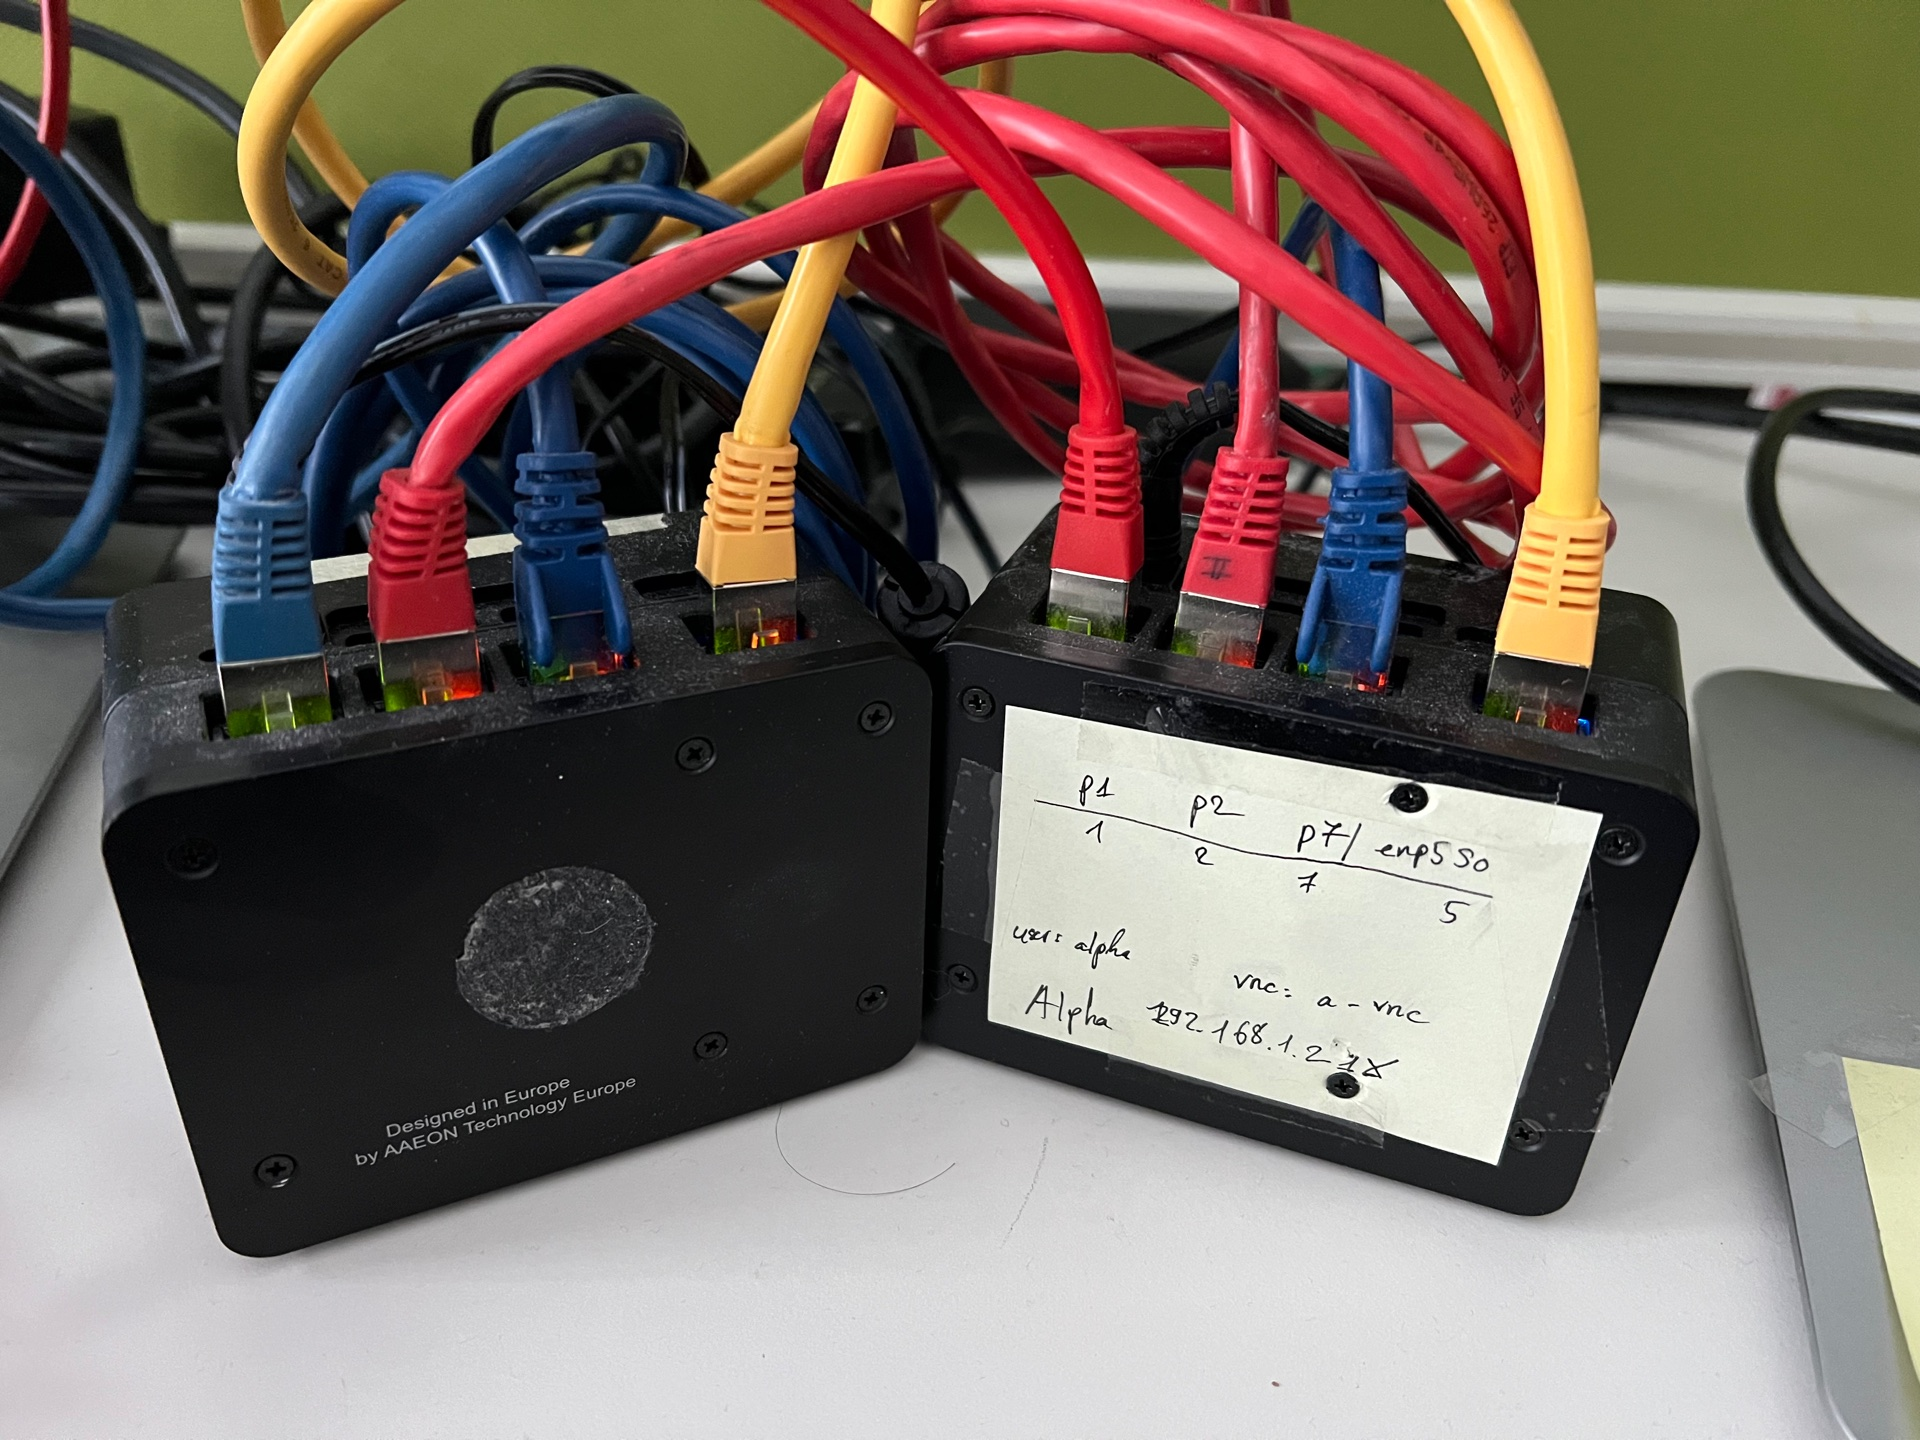
\includegraphics[width=1.0\textwidth]{upc_machines.png}
	\caption{Two UPC machines with 3 ethernet ports connected (enp3s0, enp5s0, enp7s0). Port enp1s0 is connected to workstation for remote management purpose.}
	\label{fig:plan:upc_machines}
\end{figure}


\clearpage
\section{Timeline}

\begin{sidewaysfigure}
    \centering
    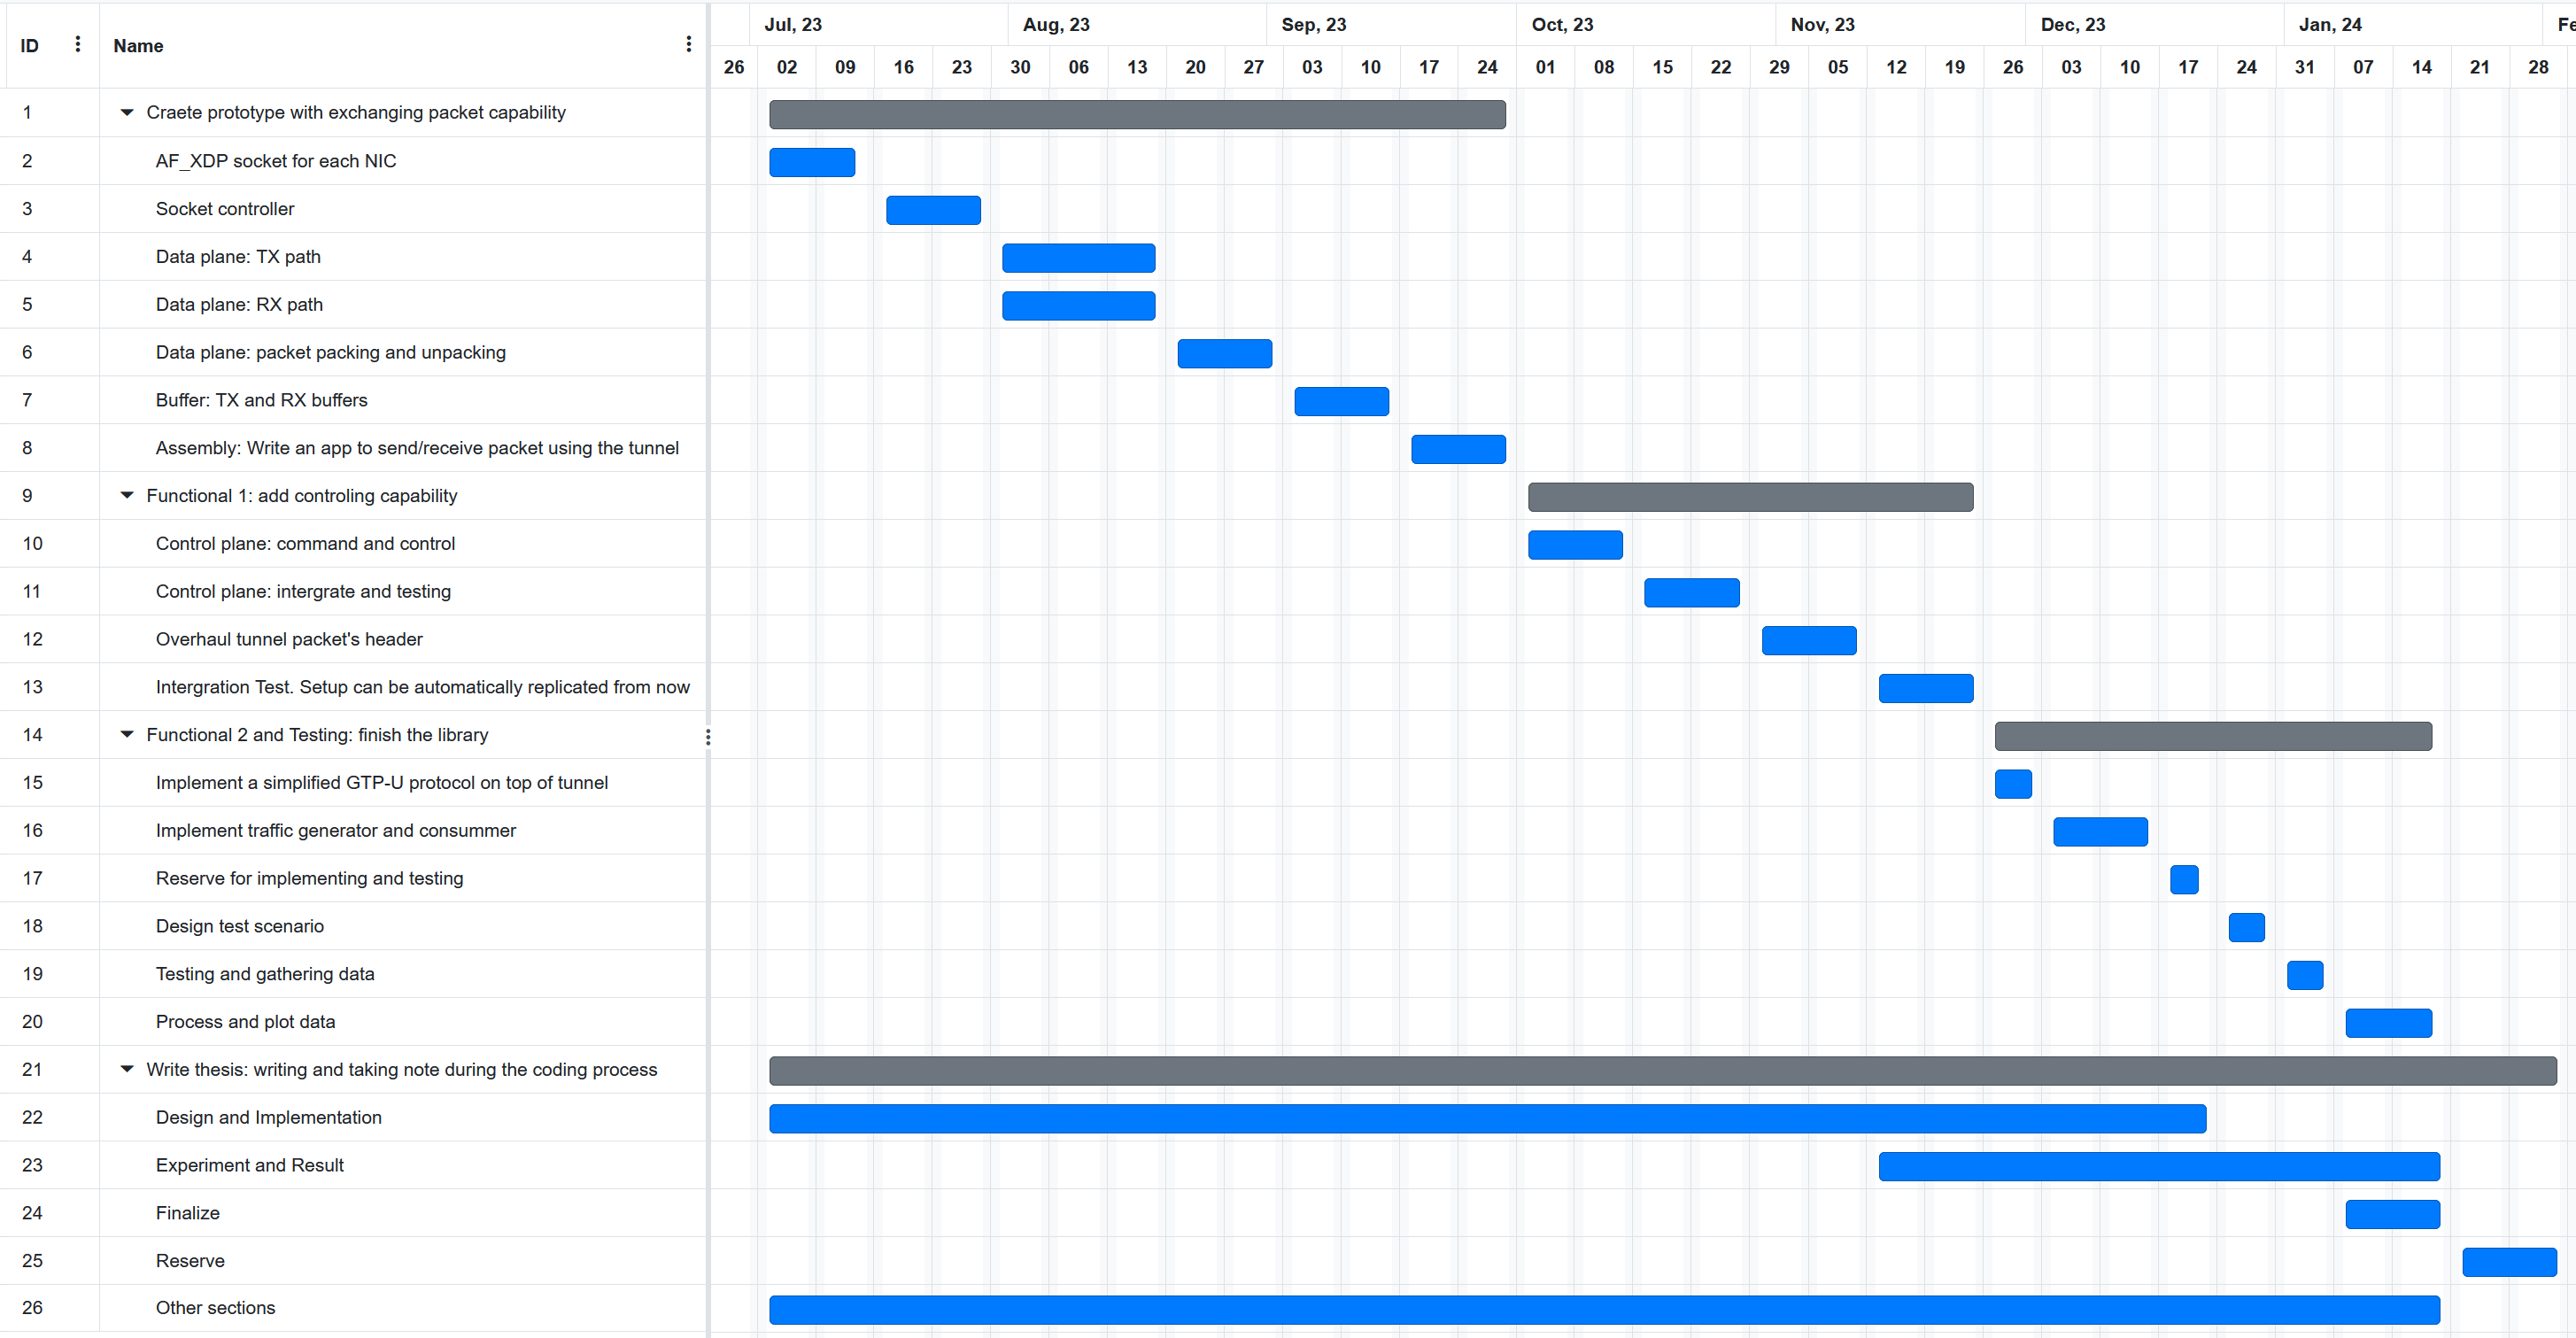
\includegraphics[width=1.0\textwidth]{resources/images/TIMELINE.PNG}
    \caption{Expected progress. The thesis can be finished in 6 months..}
  \end{sidewaysfigure}





% \begin{wrapfigure}{r}{0.2\textwidth}
%     \centering
%     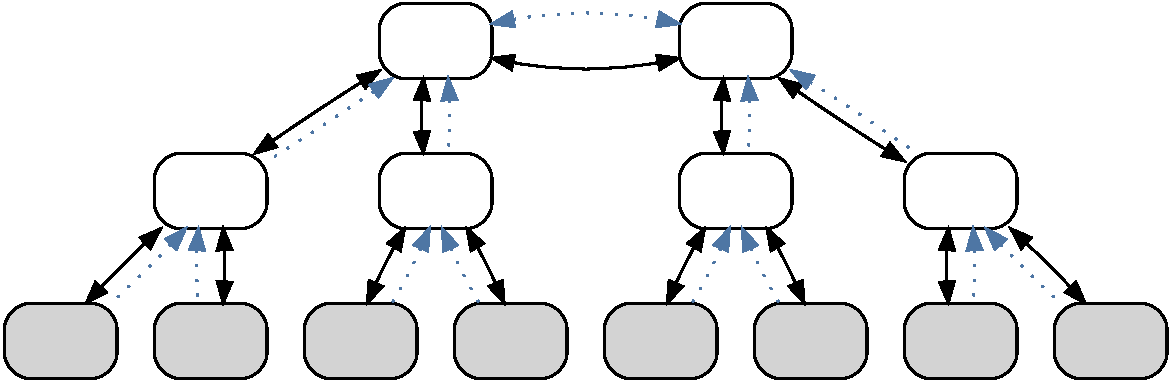
\includegraphics[width=0.2\textwidth]{resources/images/example3}
% \end{wrapfigure}

% \sidenote{Contributions}
% \todomid{write}

% \begin{figure}
%     \centering
%     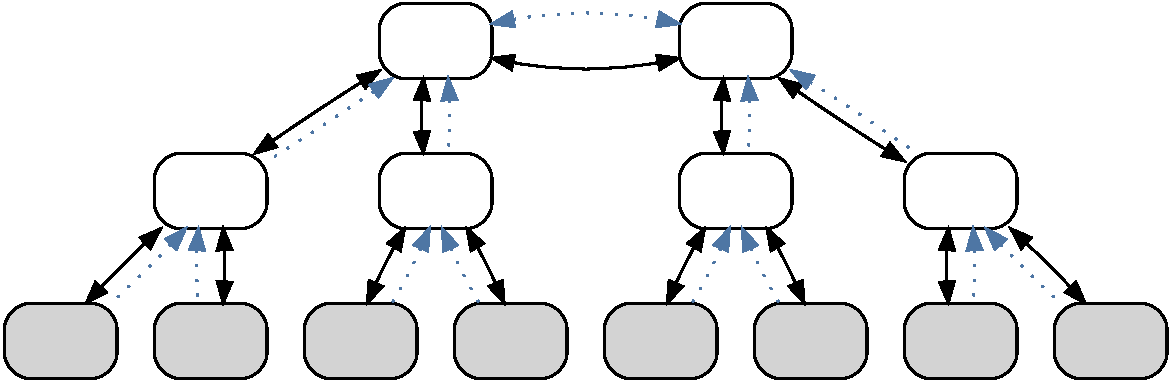
\includegraphics[width=.55\textwidth]{resources/images/example3}
%     \caption{Placement of the outlook in the structure of research}\label{fig:hourglass:outlook}
% \end{figure}

% \sidenote{Dissemination}
% \todomid{write about \Cref{fig:hourglass:outlook}}

% \section{Conclusions and Impact}

% \sidenote{Context}
% \todomid{write}

% \sidenote{Contribution 1}
% \todomid{write}

% \sidenote{Contribution 2}
% \todomid{write}

% \sidenote{Contribution 3}
% \todomid{write}

% \section{Outlook}

% \sidenote{Intro}
% \todomid{write}

% \sidenote{Application Area 1}
% \todomid{write about \Cref{fig:outlook:aa1}}

% \begin{figure}
%     \centering
%     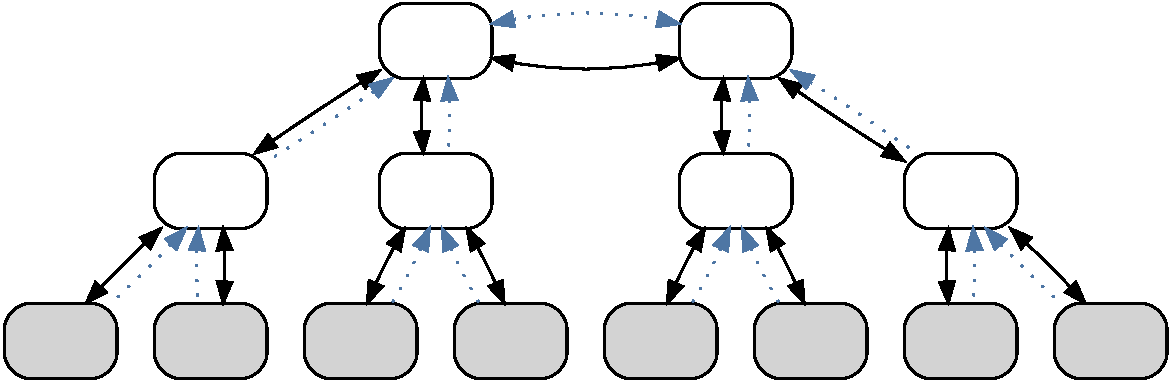
\includegraphics[width=.85\textwidth]{resources/images/example3}
%     \caption{Area 1~\cite{li2002design}}\label{fig:outlook:aa1}
% \end{figure}

% \sidenote{Application Area 2}
% \todomid{write}

% \sidenote{Application Area 3}
% \todomid{write}

% \sidenote{Application Area 4}
% \todomid{write}
